\chapter{Algorytmy ewolucyjne}
\label{cha:genetyczne}

Algorytmami ewolucyjnymi nazywne są algoytmy, które w celu przeszukania przestrzeni rozwiązań  wykorzystują mechanizmy zaczerpnięte ze zjawiska ewolucji biologicznej. Jest to ogólna nazwa dla metod takich jak algorytmy genetyczne, strategie ewolucyjne czy neuroewolucje. 

Podobnie jak opisane w rozdziale \ref{cha:pso} algorytmy rojowe, ewolucyjne również zawierają populację agentów wpływających nawzajem na siebie. Populacja agentów generowana jest losowo, wraz z pewnym zestawem cech dla każdego agenta - genotypem. Genotyp jest takim zestawem cech agenta, który umiejscawia go w pewnej przestrzeni rozwiązań, co umożliwia jego ewaluację. Podczas działania algorytmu, agenci poprzez krzyżowanie się, umieranie i rodzenie wpływają na swoje genotypy. 

Na przestrzeni lat zostało zaproponowanych wiele algorytmów bazujących na mechanizmach genetycznych, jednak wszystkie z nich opierały się na tych samych bazowych mechanizmach. Każdy z osobników populacji mógł, zmieniając swój genotyp, przybliżyć całą populację do znalezienia optymalnego rozwiązania postawionego problemu. Większość wpółczesnych rozwiązań stosuje również krzyżowanie się osobników, jako drugą główną składową działania algorytmów tego typu.

\section{Przegląd wiedzy}
\label{sec:historiagenetycznych}
Początki algorytmów ewolucyjnych sięgają lat 50 XX wieku\cite{GA1}, jednak ich idee nie były rozwijane przez wiele lat, głównie ze względu na ograniczenia sprzętowe jak i metodologiczne. Dopiero dwadzieścia lat później\cite{GA2} pojawiły się prace rozwijające modele ewolucyjne. Wtedy też zostało zaproponowane twierdzenie Hollanda o schematach, które uważane jest za podstawę wyjaśnienia algorytmów genetycznych. 

Znaczącą kwestią wpływającą na tempo rozwoju algorytmów genetycznych, było użycie techniki uwzględniającej ewolucję zarówno przez mutację jak i krzyżowanie się osobników z danej populacji. Podczas kolejnych lat badań, algorytmy tego typu zostały poszerzone o kod genetyczny pozwalający reprezentować strukturę każdego problemu.

Klasyczne algorytmy ewolucyjne działają zgodnie z algorytmem przedstawionym na diagramie \ref{fig:GAdiagram}, lub podobnie do niego. 

\begin{figure}[H]
\begin{center} 
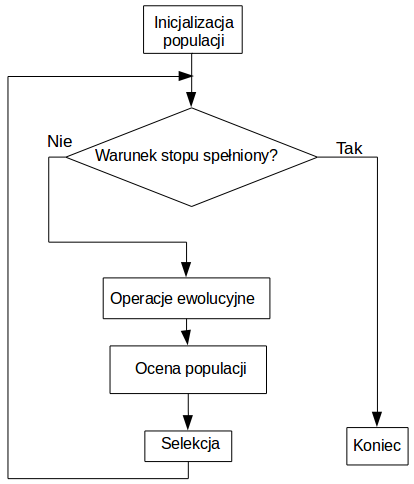
\includegraphics[scale=0.6]{tresc/pics/GAdiagram.png}
\caption{Diagram blokowy klasycznego algorytmu genetycznego}
\label{fig:GAdiagram}
\end{center}
\end{figure}

Początkowo inicjalizowana jest losowa populacja, która wykonuje między sobą zachowania ewolucyjne aż do spełnienia warunku stopu. Podczas każdej iteracji z całej populacji wybierana jest część osobników która zostanie poddana krzyżowaniu się między sobą. Następnie te osobniki poddawane są mutacji. Dla każdego z osobników wyliczana jest funkcja przystosowania, pozwalająca ocenić jakość jego genotypu.

\section{Algorytm EMAS}

Algorytm EMAS (ang. Evolutionary Multi-Agent System) jest paradygmatem obliczeniowym zaproponowanym w 1996 roku\cite{emas1}. Jest to połączenie algorytmu ewolucyjnego z systemem wieloagentowym. Idea algorytmu opiera się na koncepcji, że agenci w środowisku mogą się łączyć, reprodukować i umierać. 

Przeznaczony jest do pracy bez zachowania jakiejkolwiek globalnej wiedzy o problemie. Agenci są niezależni oraz zdolni do podejmowania własnych decyzji dotyczących ich akcji. Ta cecha sprawia, że algorytm jest łatwo skalowalny i pozwala na zrównoleglenie. 

Dziedziczenie i selekcja to dwa główne elementy algorytmów ewolucyjnych, które w algorytmie EMAS realizowane są za pomocą zjawisk śmierci i reprodukcji. Agenci o najlepszym przystosowaniu są zachowane i mogę produkować swoje potomstwo. Agenci o najgorszych parametrach są całkowicie usuwane z otoczenia. Takie zachowanie zmusza populację do ewolucji oraz poprawia jej parametry\cite{emas2}.

\subsection{Agent}
\label{sec:agentgenetyczny}
Każdy z agentów charakteryzuje się trzema parametrami:
\begin {itemize}
\item genotyp (ang. genotype)
\item dopasowanie (ang. fitness)
\item energia (ang. energy)
\end {itemize}
Genotyp agenta stanowi pojedynczą odpowiedź na zadany problem populacji. Jest to podstawa do obliczenia dopasowania. Genotyp jest cechą dziedziczoną podczas reprodukcji i ulega mutacji w procesie ewolucji. Jako zasadniczy parametr agenta jest to podstawa dla pozostałych parametrów.

Kolejną cechą jest dopasowanie, które jest liczbą reprezentującą jakość genotypu. Lepsze genotypy mają lepsze wartości dopasowania i mają większe prawdopodobieństwo aby być wybranym przy procesie reprodukcji. Sama wartość jest obliczana bezpośrednio z parametru genotypu po stworzeniu agenta. Dopasowanie danego agenta, tak samo jak jego genotyp nie zmienia sie w czasie jego życia.

Ostatnią cechą, wpływającą na sposób selekcji jest energia. Ze względu na brak globalnej wiedzy agentów, nie jest możliwa ocena ich wszystkich w tym samym czasie. Ponieważ proces ewolucji jest asynchroniczny, metody selekcji znane z klasycznych algorytmów ewolucyjnych nie mogły zostać użyte. Z tego powodu została wprowadzona energia, można opisać ten parametr jako stan agenta, który podczas interakcji może ją zyskiwać lub tracić, zależnie od jakości genotypu. Agenci z lepszym genotypem są bardziej skłonni do gromadzenia energii, jednak całkowita ilość energii w populacji jest stała.

Ponieważ agenci w algorytmie EMAS są całkowicie autonomiczni, decyzję o swoim zachowaniu podejmują na podstawie poziomu energii. Jeśli jej liczba przekracza pewien próg to będą się reprodukować, a jeśli osiągnie zero to agent umiera\cite{emas3}.


\subsection{Interakcje agentów}
Istnieją trzy możliwe działania agenta, które może podjąć w danym kroku iteracji:
\begin{itemize} 
\item śmierć (ang. death) 
\item reprodukcja (ang. reproduction) 
\item walka (ang. fight) 
\end{itemize}

Śmierć to usunięcie agenta z populacji, spowodowane jest najczęściej poprzez osiągnięcie przez danego agenta zerowego poziomu energii.

Reprodukcja jest procesem tworzenia nowych agentów. Wymaga wystąpienia jednego lub dwójki rodziców i skutkuje odpowiednio jednym lub dwójką nowo powstałych agentów. Jak zostało wspomniane w rozdziale \ref{sec:agentgenetyczny}, rozwiązanie oraz dopasowanie są stałe podczas życia agenta, więc ich wartość u rodziców się nie zmienia. Jedyną zmianą parametru jest zmniejszenie ich poziomu energii, która jest przekazywana nowopowstałym agentom. Genotypy nowo narodzonych agentów są tworzone poprzez losowe zmieszanie genotypów ich rodziców. W momencie uzyskania genotypu, możliwe jest obliczenie dopasowania danego agenta.

Walka jest działaniem odpowiedzialnym za wymianę energii. Dzięki niej, agenci o lepszym genotypie są w stanie pobrać energię od tych z gorszym. Walka sprowadza się do porównaniu dopasowania dwóch agentów i w jego efekcie transferze energii. Jest to szybki sposób porównania i nagradzania najlepszych rozwiązań.

Jak zostało wspomniane wcześniej, ilość energii jest stała w całym układzie. W wyniku reprodukcji nowo narodzony agent dostaje energię od rodziców, natomiast w przypadku walki następuje wymiana pomiędzy dwoma agentami.

\subsection{Ewolucja}

Pomimo, że proces ewolucji jest asynchorniczny można zauważyć pewien schemat zachowania, przedstawiony na rysunku \ref{fig:emasdiagram}.

\begin{figure}[H]
\begin{center} 
\includegraphics[scale=0.6]{tresc/pics/emasdiagram.png}
\caption{Operacje ewolucyjne w algorytmie EMAS}
\label{fig:emasdiagram}
\end{center}
\end{figure}

Pierwszym krokiem jest zdecydowanie jakie działania powinien podjąć agent w danej iteracji. Ponieważ nie ma żadnej wiedzy globalnej, jego decyzje opierają się wyłącznie o jego parametry. Wszyscy agenci zostają oznaczeni jaką akcję podejmą w danym kroku.

Następnie agenci są dzieleni na trzy grupy, odpowiednio dla akcji które zostaną podjęte. Ma to na celu spowodowanie współdziałania ich ze sobą. Ponieważ agenci nie wiedzą jakie działania podejmą pozostali, ten krok jest wymagany aby spowodować interakcje wewnątrz populacji.

Kolejnym krokiem jest przeprowadzenie akcji wewnątrz grup. Część agentów umiera, a część powstaje, zależnie od składu grup. W ostatnim kroku agenci są zbierani w całość, a następnie przemieszani. Ma to na celu uniknięcie ciągłej interakcji ze sobą tych samych agentów.


\subsection{Wyspy obliczeniowe}
Populacją nazywany jest cały zbiór agentów, Jej początkowy rozmiar jest parametryzowany i zmienia się w czasie wykonywania programu. Interakcje wewnątrz populacji nie odbiegają zbytnio od większości algorytmów ewolucyjnych.

Podczas pojedynczego przebiegu programu można utworzyć wiele różnych populacji nazywanych wyspami\cite{emas3}, zmieniających się niezależnie w tym samym czasie. 

Poprzez wprowadzenie migracji między różnymi wyspami, jest możliwe eksportowanie pewnych rozwiązań pomiędzy wyspami, co ma pozytywny wpływ na ogólną wydajność. Dobre rozwiązanie opracowane w jednej populacji może być wprowadzone do innej, powodując modyfikację genotypu. 

Wprowadzenie wysp obliczeniowych dodaje każdemu agentowi dodatkową akcję jaką może podjąć, a mianowicie migrację. Jak wszystkie pozostałe akcje, zależna jest ona od wartości energii danego agenta.



